\chapter{A-A WEAPONS}
\thumbtab{A-A}{5}
\localtableofcontents
\cleardoublepage

\section{AIR-TO-AIR GUNNERY}

\subsection{M-61 CANNON}

\begin{tcoloritemize}
    \blueitem{M-61}{
    Internally mounted, high fire-rate, 20mm rotary ``Gattling'' cannon.
    In service since 1959

    \begin{subitemize}
        \item \textbf{Fire Rate} --- 6000rpm
        \item \textbf{Round Size} --- 20mm
        \item \textbf{Ammo Capacity} --- 510 rounds
    \end{subitemize}}
\end{tcoloritemize}

\begin{figure}[htbp]
    \centering
    \fbox{
    \begin{minipage}[t][75mm][t]{100mm}
        \center{\large\textbf{M-61 OVERVIEW}}
        \begin{itemize}
            \item Some kind of overview figure
            \item maybe showing side on profile of the weapon?
        \end{itemize}
    \end{minipage}
    }
    \caption{M-61 Cannon}
\end{figure}
    
\begin{tcoloritemize}
    \blueitem{Ammunition Types}{
    \begin{subitemize}
        \item \textbf{HEI} --- \textbf{H}igh \textbf{E}xplosive \textbf{I}ncendiary
        \item \textbf{HEI-T} --- \textbf{H}igh \textbf{E}xplosive \textbf{I}ncendiary-\textbf{T}racer
        \item \textbf{AP} --- \textbf{A}rmor \textbf{P}iercing
        \item \textbf{TP} --- \textbf{T}arget \textbf{P}ractice
        \item \textbf{SAPHEI} --- \textbf{S}emi \textbf{A}rmor \textbf{P}iercing \textbf{H}igh \textbf{E}xplosive \textbf{I}ncendiary
    \end{subitemize}}
    \blueitem{Select GUN}{
    Via Dogfight --- AIM-9 \& GUN automatically selected

    \begin{subenumerate}
        \item \textbf{DGFT/MSL OVRD} \dotfill \textbf{DGFT}
    \end{subenumerate}

    Via A-A Master Mode

    \begin{subenumerate}
        \item \textbf{Master Mode} \dotfill \textbf{A-A}
        \item \textbf{SMS OSB 1} \dotfill \textbf{Cycle to GUN}
    \end{subenumerate}}
\end{tcoloritemize}

\subsubsection{SMS CONTROLS}

\begin{tcoloritemize}
    \blueitem{Operating Mode}{\textbf{OSB 1} cycles A-A modes, should display \textbf{GUN}}
    \blueitem{Sub-Mode}{\textbf{OSB 2} cycles gunsight modes
    
    \begin{subitemize}
        \item \textbf{EEGS} --- \textbf{E}nhanced \textbf{E}nvelope \textbf{G}un\textbf{S}ight \\
        \textbf{See \Cref{subsec:eegssymb}}
    \end{subitemize}}
    \blueitem{Rounds \break Remaining}{Indicates number of rounds remaining in 10s}
\end{tcoloritemize}

\begin{figure}[htbp]
    \centering
    \fbox{
    \begin{minipage}[t][75mm][t]{100mm}
        \center{\large\textbf{MFD --- SMS --- GUN CONTROLS}}
        \begin{itemize}
            \item show sms gun page
            \item label each of the relevant controls explained in text
        \end{itemize}
    \end{minipage}
    }
    \caption{MFD SMS Gun Controls}
\end{figure}

\subsubsection{EEGS SYMBOLOGY}
\label{subsec:eegssymb}
\begin{tcoloritemize}
    \blueitem{EEGS}{\textbf{E}nhanced \textbf{E}nvelope \textbf{G}un\textbf{S}ight
    \begin{subitemize}
        \item \textbf{Provides multiple levels of symbology depending on presence of radar lock}
    \end{subitemize}}
    \blueitem{Level I}{Backup mode displaying only boresight cross in event of INS failure}
    \blueitem{Level II}{Operating mode prior to radar lock

    \begin{subitemize}
        \item \textbf{Boresight Cross} --- shows where gun / aircraft is pointed
        \item \textbf{EEGS Funnel}
        \begin{itemize}
            \item displays path of rounds through space
            \item funnel is of set width to judge distance --- adjust width to target wingspan, stabilize edges of funnel on wingtips and fire
        \end{itemize}
        \item \textbf{MGRS} --- \textbf{M}ultiple \textbf{R}eference \textbf{G}un\textbf{S}ight
        \begin{itemize}
            \item 5 line-segments pointing towards boresight
            \item reference for high aspect snap shots (placeing target on MGRS line should have it fly through gun cross)
        \end{itemize}
    \end{subitemize}
    
    Reference symbology in \cref{fig:aaweap:m61:eegslvl2} and \cref{fig:aaweap:m61:funnelpipper}
    }
    \blueitem{Level III / IV}{Intermediate modes during radar lock acquisition}
    \blueitem{Level V}{Operating mode with radar lock. Level II symbology is retained with additional elements
    
    \begin{subitemize}
        \item \textbf{Level V Pipper}
        \begin{itemize}
            \item gunfire solution --- stabilize pipper on target and fire
            \item contains additional range/aspect cues
        \end{itemize}
        \item \textbf{Range Caret}
        \begin{itemize}
            \item displayed on \underline{inside} edge of level V pipper
            \item unwinds from 12 o'clock at 12'000ft counter-clockwise
        \end{itemize}
        \item \textbf{Aspect Caret} 
        \begin{itemize}
            \item displayed on \underline{outside} edge of level V pipper
        \end{itemize}
        \item \textbf{T-Symbol}
        \begin{itemize}
            \item \textbf{``--- + ---'' 1G Pipper} --- lead angle for non-maneuvering target,
            flanking horizontal lines indicate out-of-plane maneuver potential of target
            \item \textbf{``---'' Max-G Pipper} --- lead angle for target pulling max-G towards you
        \end{itemize}
        \item \textbf{BATR} --- \textbf{B}ullets \textbf{A}t \textbf{T}arget \textbf{R}ange
        \begin{itemize}
            \item displayed once rounds have been fired
            \item dissappears after last round has passed beyond target range
            \item useful to evaluate shots (also for training)
        \end{itemize}
    \end{subitemize}
    
    Reference symbology in \cref{fig:aaweap:m61:eegslvl5} and \cref{fig:aaweap:m61:funnelpipper}
    }
\end{tcoloritemize}

\begin{figure}[htbp]
    \centering
    \fbox{
    \begin{minipage}[t][75mm][t]{100mm}
        \center{\large\textbf{HUD --- EEGS LVL II}}
        \begin{itemize}
            \item show EEGS LVL II symbology of the HUD
            \item maybe with a simiplified target outline ``mid pull'' in the funnel?
            \begin{itemize}
                \item if don't have target here maybe put in marginfig below? (just show funnel with target at correct point to shoot)
                \item alternatively, maybe have separate figure just showing target in funnel here? (could be reused as marginfig below)
            \end{itemize}
        \end{itemize}
    \end{minipage}
    }
    \caption{EEGS LVL II HUD Symbology}
    \label{fig:aaweap:m61:eegslvl2}
\end{figure}

\begin{figure}[htbp]
    \centering
    \fbox{
    \begin{minipage}[t][75mm][t]{100mm}
        \center{\large\textbf{HUD --- EEGS LVL V}}
        \begin{itemize}
            \item show EEGS LVL V symbology of the HUD
            \item maybe with a simiplified target outline ``mid pull'' in the funnel?
            \begin{itemize}
                \item more necessary here since lvl V relies on having a lock
                \item maybe have separate figure just showing lvl 5 target pipper since there is a lot going on (could be reuses as marginfig below)
            \end{itemize}
        \end{itemize}
    \end{minipage}
    }
    \caption{EEGS LVL V HUD Symbology}
    \label{fig:aaweap:m61:eegslvl5}
\end{figure}

\begin{figure}[htbp]
    \centering
    \fbox{
    \begin{minipage}[t][50mm][t]{100mm}
        \center{\large\textbf{EEGS Funnel \& LVL V Pipper}}
        \begin{itemize}
            \item show both funnel and pipper as subfigs
            \item include target outline in firing position
            \item clearly mark level 5 pipper symbology elements
            \begin{itemize}
                \item batr
                \item range cue
                \item aspect
            \end{itemize}
        \end{itemize}
    \end{minipage}
    }
    \caption{EEGS Funnel \& Level V Pipper}
    \label{fig:aaweap:m61:funnelpipper}
\end{figure}

\marginfigeometry

\subsubsection{GUN SELECTION}
\begin{checklistitemize}
    \blueitem{Via Dogfight}{(GUN automatically selected)
    \begin{subenumerate}
        \item \textbf{DGFT/MSL OVRD} \dotfill \textbf{DGFT}
    \end{subenumerate}}
    \blueitem{Via A-A Master Mode}{
    \begin{subenumerate}
        \item \textbf{Master Mode} \dotfill \textbf{A-A}
        \item \textbf{SMS OSB 1} \dotfill \textbf{Cycle to GUN}
    \end{subenumerate}}
    \blueitem{EEGS Symbology}{Verify
    \begin{subitemize}
        \item \textbf{EEGS Level II} appears if no lock present
        \item \textbf{EEGS Level V} appears if target locked
    \end{subitemize}}
\end{checklistitemize}

\subsubsection{EEGS LVL II EMPLOYMENT --- NO RADAR}
\begin{checklistenumerate}
    \blueitem{Prerequisites}{
    \begin{subitemize}
        \item \textbf{RF Switch} \dotfill \textbf{SILENT} \\
        \hfill (if desired, completely silences radar)
        \item \textbf{Selected Weapon} \dotfill \textbf{GUN}
        \item \textbf{Master Arm} \dotfill \textbf{ARM}
    \end{subitemize}}
    \blueitem{Acquire Firing Solution}{
    \marginpar{
        \captionsetup{type=figure}
        \fbox{
            \begin{minipage}[t][40mm][t]{\marginparwidth}
                \center{\textbf{EEGS Funnel}}
                \begin{itemize}[leftmargin=1em]
                    \item show funnel on target
                    \item potentially reuse from above
                \end{itemize}
            \end{minipage}
        }
        \caption{EEGS Funnel}
    }

    \smallskip
    Using EEGS funnel

    \begin{subenumerate}
        \item \textbf{EEGS Funnel} \dotfill \textbf{Stabilized On-Target}
        \item \textbf{Funnel Lines} \dotfill \textbf{On target wingtips}
    \end{subenumerate}
    
    \marginpar{
        \captionsetup{type=figure}
        \fbox{
            \begin{minipage}[t][40mm][t]{\marginparwidth}
                \center{\textbf{MGRS Lines}}
                \begin{itemize}[leftmargin=1em]
                    \item show MGRS line on target
                    \item not sure if this fig is necessary
                    \item maybe could modify fig from above
                \end{itemize}
            \end{minipage}
        }
        \caption{MGRS Lines}
    }
    Using MGRS lines
    
    \begin{subenumerate}
        \item \textbf{MGRS Line} \dotfill \textbf{Aligned with target}
    \end{subenumerate}}
    \blueitem{Fire Gun}{
    \begin{subenumerate}
        \item \textbf{TRIGGER} \dotfill \textbf{2nd Detent}
        \item Adjust lead to achieve desired effects
    \end{subenumerate}}
\end{checklistenumerate}

\subsubsection{EEGS LVL V EMPLOYMENT --- RADAR}

\begin{checklistenumerate}
    \blueitem{Prerequisites}{
    \begin{subitemize}
        \item \textbf{FCR Switch} \dotfill \textbf{FCR}
        \item \textbf{RF Switch} \dotfill \textbf{NORM}
        \item \textbf{Selected Weapon} \dotfill \textbf{GUN}
        \item \textbf{Master Arm} \dotfill \textbf{ARM}
    \end{subitemize}}
\end{checklistenumerate}

\clearpage

\begin{checklistenumerate}[resume]
    \blueitem{Radar Acquisition}{ACM selected automatically in \textbf{DGFT} mode, \textbf{see \Cref{subsec:acm}}
    
    \begin{subenumerate}
        \item \textbf{ACM Submode} \dotfill \textbf{As desired}
        \item Maneuver to place target in radar scan volume
    \end{subenumerate}}
    \blueitem{Acquire Firing Solution}{
    \marginpar{
        \captionsetup{type=figure}
        \fbox{
            \begin{minipage}[t][40mm][t]{\marginparwidth}
                \center{\textbf{EEGS Level V Pipper}}
                \begin{itemize}[leftmargin=1em]
                    \item show pipper on target
                    \item potentially reuse from above
                \end{itemize}
            \end{minipage}
        }
        \caption{EEGS Level V Pipper}
    }
    \begin{subenumerate}
        \item \textbf{Pipper} \dotfill \textbf{Stabilized On-Target}
    \end{subenumerate}}
    \blueitem{Fire Gun}{
    \begin{subenumerate}
        \item \textbf{TRIGGER} \dotfill \textbf{2nd Detent}
        \item Adjust lead to achieve desired effects
    \end{subenumerate}}
\end{checklistenumerate}

\subsubsection{ADJUST EEGS FUNNEL WIDTH}

\begin{checklistenumerate}
    \blueitem{Open DED MAN Page}{
    \begin{subenumerate}
        \item \textbf{ICP LIST Button} \dotfill \textbf{Press}
        \item \textbf{DED MAN Page} \dotfill \textbf{Open (5)} 
    \end{subenumerate}}
    \blueitem{Adjust Wingspan}{
    \begin{subenumerate}
        \item \textbf{WSPAN} \dotfill \textbf{Selected}
        \item \textbf{Desired Value} \dotfill Input on ICP, \textbf{ENTR}
        \item \textbf{WSPAN} \dotfill Verify as desired
    \end{subenumerate}}
\end{checklistenumerate}

\marginfigrestore

\section{AIR-TO-AIR MISSILES}

\subsection{AIM-9 SIDEWINDER}

\begin{figure}[htbp]
    \centering
    \fbox{
    \begin{minipage}[t][75mm][t]{100mm}
        \center{\large\textbf{AIM-9 OVERVIEW}}
        \begin{itemize}
            \item Some kind of overview figure
            \item maybe showing side on profile of the weapon?
        \end{itemize}
    \end{minipage}
    }
    \caption{AIM-9 Sidewinder}
\end{figure}

\begin{tcoloritemize}
    \blueitem{AIM-9 \break Sidewinder}{
    Short-range, fire-and-forget ``dogfight'' missile. First entered service in 1956

    \begin{subitemize}
        \item \textbf{Guidance} --- IR-guided (\textbf{Fox 2})
        \item \textbf{Range} --- min: \textasciitilde3000ft, max: \textasciitilde10-20nm
    \end{subitemize}}
    \blueitem{Variants}{
    \begin{subitemize}
        \item \textbf{9M} --- IR-guided, short range, all-aspect
        \item \textbf{9X} --- HOBS (\textbf{H}igh \textbf{O}ff-\textbf{B}ore\textbf{S}ight) capable, thrust-vectored, all-aspect
    \end{subitemize}}
    \blueitem{Acquisition / Cueing Modes}{
    \begin{subitemize}
        \item Acquisition with own missile seeker (BORE)\\
        \hyperref[subsec:aim9:bore]{\textbf{See \Cref{subsec:aim9:bore}}}
        \item Seeker slaved to radar track LOS (SLAVE)\\
        \hyperref[subsec:aim9:slave]{\textbf{See \Cref{subsec:aim9:slave}}}
        \item Seeker cued with HMD LOS \\
        \textbf{See\Cref{subsec:aim9:hmcs} for BORE}
    \end{subitemize}}
    \blueitem{Select AIM-9}{
    Via Dogfight --- AIM-9 \& GUN automatically selected

    \begin{subenumerate}
        \item \textbf{DGFT/MSL OVRD} \dotfill \textbf{DGFT}
        \item \textbf{Selected Weapon (OSB 7)} \dotfill Verify \textbf{9LM / 9X}
    \end{subenumerate}

    Via Missile Override

    \begin{subenumerate}
        \item \textbf{DGFT/MSL OVRD} \dotfill \textbf{OVRD}
        \item \textbf{Selected Weapon (SMS OSB 7)} \dotfill \textbf{9LM / 9X}
    \end{subenumerate}

    Via A-A Master Mode

    \begin{subenumerate}
        \item \textbf{Master Mode} \dotfill \textbf{A-A}
        \item \textbf{Operating Mode (SMS OSB 1)} \dotfill Verify \textbf{AAM}
        \item \textbf{Selected Weapon (SMS OSB 7)} \dotfill \textbf{9LM / 9X}
    \end{subenumerate}
    
    Selected weapon can also be cycled with \textbf{NWS/MSL Step depress (long)}
    }
\end{tcoloritemize}
    
\subsubsection{SMS CONTROLS}

\begin{tcoloritemize}
    \blueitem{SPOT / SCAN}{
    \textbf{OSB 2} controls seeker field of view
    \begin{subitemize}
        \item \textbf{SPOT} --- Narrow, increased detection range
        \item \textbf{SCAN} --- Wide, decreased detection range
    \end{subitemize}}
    \blueitem{Selected Weapon}{
    \textbf{OSB 7} cycles through available A-A weapon types
    
    \medskip
    Selected weapon can also be cycled with \textbf{NWS/MSL Step depress (long)}
    }
    \blueitem{WARM / COOL}{
    \textbf{OSB 8} controls seeker cooling status

    \begin{subitemize}
        \item \textbf{COOL} ---  increases seeker sensitivity, should be set prior to engagement
        \item Set automatically for \textbf{DGFT} \& \textbf{MSL OVRD}
    \end{subitemize}}
    \blueitem{Selected Station}{
    \textbf{OSB 10 / 16} select/cycle availabel missile pylons
    
    \medskip
    Selected station can also be cycled with \textbf{NWS/MSL Step depress (short)}
    }
    \blueitem{SLAVE / BORE}{
    \textbf{OSB 19} controls seeker line of sight

    \begin{subitemize}
        \item \textbf{BORE} --- \hyperref[subsec:aim9:bore]{\textbf{See \Cref{subsec:aim9:bore}}}
        \begin{itemize}
            \item Acquisition with own missile seeker
            \item Or cued with HMD (if powered)
            \item \textbf{Does NOT require FCR}
        \end{itemize}
        \item \textbf{SLAVE} --- \hyperref[subsec:aim9:slave]{\textbf{See \Cref{subsec:aim9:slave}}}
        \begin{itemize}
            \item Seeker slaved to radar track LOS
            \item Typically via ACM Modes
        \end{itemize}
    \end{subitemize}}
\end{tcoloritemize}

\begin{figure}[htbp]
    \centering
    \fbox{
    \begin{minipage}[t][75mm][t]{100mm}
        \center{\large\textbf{MFD --- SMS --- AIM-9 CONTROLS}}
        \begin{itemize}
            \item show sms aim-9 page
            \item label each of the relevant controls explained in text
        \end{itemize}
    \end{minipage}
    }
    \caption{MFD SMS AIM-9 Controls}
\end{figure}

\clearpage

\subsubsection{SYMBOLOGY}
\begin{tcoloritemize}
    \blueitem{MFD Symbology}{Reference \textbf{\underline{insert reference to aim-120 subsubsec}}}
    \blueitem{HUD/HMD \break Symbology}{
    \begin{subitemize}
        \item \textbf{Missile Diamond} --- AIM-9 seeker line-of-sight
        \begin{itemize}
            \item displayed on HUD \& HMD
            \item marked with \textbf{X} if beyond seeker limits
        \end{itemize}
        \item \textbf{Missile Reticle} --- AIM-9 seeker field-of-view
        \begin{itemize}
            \item displayed on HUD only
            \item size reflects \textbf{SPOT/SCAN} setting 
        \end{itemize}
        \item \textbf{Dynamic Aiming Cross} --- HMD line-of-sight
    \end{subitemize}

    Reference symbology in \cref{fig:aaweap:aim9:hudhmdsymb}

    \begin{subitemize}
        \item \textbf{DLZ} --- \textbf{D}ynamic \textbf{L}aunch \textbf{Z}one
        \begin{itemize}
            \item \textbf{\underline{insert reference to aim-120 subsubsec}}
        \end{itemize}
    \end{subitemize}
    }
\end{tcoloritemize}

\begin{figure}[htbp]
    \centering
    \fbox{
    \begin{minipage}[t][75mm][t]{100mm}
        \center{\large\textbf{HUD/HMD --- AIM-9 Symbology}}
        \begin{itemize}
            \item show hud/hmd with aim-9 in use 
            \item clearly indicate missile diamond/reticle and dynamic aiming cross
            \item maybe show several versions?
            \begin{itemize}
                \item 1 with missile reticle from HUD?
                \item 1 with missile diamond latchedon aiming cross?
                \item 1 with diamond on target?
                \item 1 with \textbf{X}?
            \end{itemize}
            or some subset of those?
            \item can reuse these in marginfigs below?
        \end{itemize}
    \end{minipage}
    }
    \caption{HUD/HMD AIM-9 Symbology}
    \label{fig:aaweap:aim9:hudhmdsymb}
\end{figure}

\marginfigeometry

\subsubsection{AIM-9 SELECTION}
\begin{checklistitemize}
    \blueitem{Via DGFT}{(AIM-9 selected automatically)
    \begin{subenumerate}
        \item \textbf{DGFT/MSL OVRD} \dotfill \textbf{DGFT}
    \end{subenumerate}}
    \blueitem{Via MSL OVRD}{
    \begin{subenumerate}
        \item \textbf{DGFT/MSL OVRD} \dotfill \textbf{MSL OVRD}
        \item \textbf{Selected Weapon} \dotfill \textbf{9M/9X}
        \begin{itemize}
            \item \textbf{SMS OSB 7} --- \textbf{Press}
            \item or \textbf{NWS/MSL STEP} --- \textbf{Press (long)}
        \end{itemize}
    \end{subenumerate}}
    \blueitem{Via A-A Master Mode}{
    \begin{subenumerate}
        \item \textbf{Master Mode} \dotfill \textbf{A-A}
        \item \textbf{SMS OSB 1} \dotfill \textbf{Verify AAM} (default)
        \item \textbf{Selected Weapon} \dotfill \textbf{9M/9X}
        \begin{itemize}
            \item \textbf{SMS OSB 7} --- \textbf{Press}
            \item or \textbf{NWS/MSL STEP} --- \textbf{Press (long)}
        \end{itemize}
    \end{subenumerate}}
\end{checklistitemize}

\subsubsection{BORE EMPLOYMENT --- NO RADAR}
\label{subsec:aim9:bore}
\begin{checklistenumerate}
    \blueitem{Prerequisites}{
    \begin{subitemize}
        \item \textbf{RF Switch} \dotfill \textbf{SILENT} \\
        \hfill (if desired, completely silences radar)
        \item \textbf{Selected Weapon} \dotfill \textbf{9M/9X}
        \item \textbf{SLAVE/BORE} \dotfill \textbf{BORE}
        \item \textbf{WARM/COOL} \dotfill Verify \textbf{COOL}
        \item \textbf{Master Arm} \dotfill \textbf{ARM}
    \end{subitemize}}
    \blueitem{AIM-9 Track Acquisition}{
    \marginpar{
        \captionsetup{type=figure}
        \fbox{
            \begin{minipage}[t][40mm][t]{\marginparwidth}
                \center{\textbf{AIM-9 Track}}
                \begin{itemize}[leftmargin=1em]
                    \item show missile reticle
                    \item show diamond latched to symbolic target (outline)
                \end{itemize}
            \end{minipage}
        }
        \caption{AIM-9 Track}
    }
    \begin{subenumerate}
        \item \textbf{Missile Reticle} \dotfill \textbf{On-Target}
        \item \textbf{Sidewinder Audio} \dotfill \textbf{Lock Tone}
        \item \textbf{CAGE/UNCAGE} \dotfill \textbf{Press}
        \item \textbf{Missile Diamond} \dotfill verify latched to target
    \end{subenumerate}}
    \blueitem{Fire Missile}{
    \begin{subenumerate}
        \item Maneuver into firing position
        \item \textbf{Sidewinder Audio} \dotfill \textbf{Lock Tone}
        \item \textbf{WPN REL} \dotfill \textbf{Depress}
    \end{subenumerate}}
\end{checklistenumerate}

\clearpage

\subsubsection{HMCS BORE EMPLOYMENT --- NO RADAR}
\label{subsec:aim9:hmcs}
\begin{checklistenumerate}
    \blueitem{Prerequisites}{
    \begin{subitemize}
        \item \textbf{HMD SYMB. INT} \dotfill \textbf{INT}
        \item \textbf{RF Switch} \dotfill \textbf{SILENT} \\
        \hfill (if desired, completely silences radar)
        \item \textbf{Selected Weapon} \dotfill \textbf{9M/9X}
        \item \textbf{SLAVE/BORE} \dotfill \textbf{BORE}
        \item \textbf{WARM/COOL} \dotfill Verify \textbf{COOL}
        \item \textbf{Master Arm} \dotfill \textbf{ARM}
    \end{subitemize}}
    \blueitem{AIM-9 Track Acquisition}{
    \marginpar{
        \captionsetup{type=figure}
        \fbox{
            \begin{minipage}[t][40mm][t]{\marginparwidth}
                \center{\textbf{AIM-9 HMD Track}}
                \begin{itemize}[leftmargin=1em]
                    \item show missile diamond \& dynamic aiming cross
                    \item show diamond latched to symbolic target?
                \end{itemize}
            \end{minipage}
        }
        \caption{AIM-9 HMD Track}
    }
    \marginpar{
        \captionsetup{type=figure}
        \fbox{
            \begin{minipage}[t][40mm][t]{\marginparwidth}
                \center{\textbf{AIM-9 HMD LOS}}
                \begin{itemize}[leftmargin=1em]
                    \item show missile diamond out of HMD limits
                    \item can probably reuse from above
                \end{itemize}
            \end{minipage}
        }
        \caption{HMD beyond seeker limits}
    }
    \begin{subenumerate}
        \item Maneuver to place target within AIM-9 seeker limits
        \item \textbf{HMD Aiming Cross} \dotfill \textbf{On-Target}
    \end{subenumerate}

    Missile diamond follows aiming cross (within seeker limits)

    \begin{subenumerate}[start=3]
        \item \textbf{Sidewinder Audio} \dotfill \textbf{Lock Tone}
        \item \textbf{CAGE/UNCAGE} \dotfill \textbf{Press}
        \item \textbf{Missile Diamond} \dotfill verify latched to target
    \end{subenumerate}}
    \blueitem{Fire Missile}{
    \begin{subenumerate}
        \item Maneuver into firing position
        \item \textbf{Sidewinder Audio} \dotfill \textbf{Lock Tone}
        \item \textbf{WPN REL} \dotfill \textbf{Depress}
    \end{subenumerate}}
\end{checklistenumerate}

\begin{figure}[htbp]
    \centering
    \fbox{
    \begin{minipage}[t][40mm][t]{75mm}
        \center{\large\textbf{AIM-9 Envelope}}
        \begin{itemize}
            \item show overhead missile envelope around symbolic target?
            \item this is really a stretch goal \dots
        \end{itemize}
    \end{minipage}
    }
    \caption{AIM-9 Firing envelope}
    \label{fig:aaweap:aim9:envelope}
\end{figure}

\clearpage

\subsubsection{SLAVE EMPLOYMENT --- RADAR}
\label{subsec:aim9:slave}
\begin{checklistenumerate}
    \blueitem{Prerequisites}{
    \begin{subitemize}
        \item \textbf{FCR Switch} \dotfill \textbf{FCR}
        \item \textbf{RF Switch} \dotfill \textbf{NORM}
        \item \textbf{HMD SYMB. INT} \dotfill As desired
        \item \textbf{Selected Weapon} \dotfill \textbf{9M/9X}
        \item \textbf{SLAVE/BORE} \dotfill Verify \textbf{SLAVE}
        \item \textbf{WARM/COOL} \dotfill Verify \textbf{COOL}
        \item \textbf{Master Arm} \dotfill \textbf{ARM}
    \end{subitemize}}
    \blueitem{Radar Acquisition}{ACM selected automatically in \textbf{DGFT} mode, \textbf{see \Cref{subsec:acm}}
    \marginpar{
        \captionsetup{type=figure}
        \fbox{
            \begin{minipage}[t][40mm][t]{\marginparwidth}
                \center{\textbf{HMD BORE Symbology}}
                \begin{itemize}[leftmargin=1em]
                    \item show HMD BORE circle
                    \item show symbolic target (outline)
                    \item can reuse from radar chapter
                \end{itemize}
            \end{minipage}
        }
        \caption{HMD BORE Symbology}
    }
    
    \medskip
    For demonstration we will use \textbf{ACM BORE Submode} with HMD
    
    \begin{subenumerate}
        \item \textbf{FCR Mode} \dotfill \textbf{ACM}
        \item \textbf{TMS} \dotfill \textbf{FWD}
        \item \textbf{Target} \dotfill \textbf{In HMD BORE Symbol}
        \item \textbf{Radar} \dotfill wait for \textbf{STT Lock}
    \end{subenumerate}
    
    Can also lock from CRM, \textbf{see \Cref{subsec:crm}}
    }
    \blueitem{AIM-9 Track Acquisition}{
    \marginpar{
        \captionsetup{type=figure}
        \fbox{
            \begin{minipage}[t][40mm][t]{\marginparwidth}
                \center{\textbf{AIM-9 Radar Track}}
                \begin{itemize}[leftmargin=1em]
                    \item show radar target designator box
                    \item show diamond latched to target designator box
                \end{itemize}
            \end{minipage}
        }
        \caption{AIM-9 Radar Track}
    }
    \begin{subenumerate}
        \item \textbf{CAGE/UNCAGE} \dotfill \textbf{Press}
        \item \textbf{Sidewinder Audio} \dotfill \textbf{Lock Tone}
        \item \textbf{Missile Diamond} \dotfill verify latched to target
    \end{subenumerate}}
    \blueitem{Fire Missile}{
    \marginpar{
        \captionsetup{type=figure}
        \fbox{
            \begin{minipage}[t][60mm][t]{\marginparwidth}
                \center{\textbf{AIM-9 DLZ}}
                \begin{itemize}[leftmargin=1em]
                    \item show DLZ and indicate in-range symbology
                    \item can probably just reuse from aim-120
                    \item maybe link to explanation of dlz?
                \end{itemize}
            \end{minipage}
        }
        \caption{In-range DLZ}
    }
    \begin{subenumerate}
        \item Maneuver into firing position
        \item \textbf{DLZ} \dotfill indicates \textbf{In-Range}
        \item \textbf{Sidewinder Audio} \dotfill \textbf{Lock Tone}
        \item \textbf{WPN REL} \dotfill \textbf{Depress}
    \end{subenumerate}}
\end{checklistenumerate}

\marginfigrestore 

\subsection{AIM-120 AMRAAM}
\begin{figure}[htbp]
    \centering
    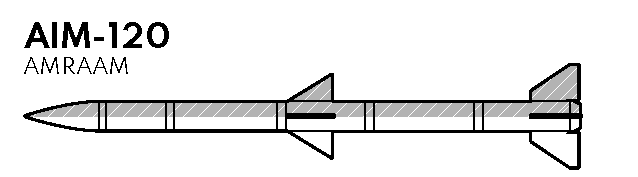
\includegraphics[
            width = 108mm,
    ]{F16_aaweapons_amraam_overview_v01.pdf}
    \fbox{
    \begin{minipage}[t][25mm][t]{100mm}
        \center{\large\textbf{AIM-120 OVERVIEW}}
        \begin{itemize}
            \item Some kind of overview figure
        \end{itemize}
    \end{minipage}
    }
    \caption{AIM-120 AMRAAM}
\end{figure}

\begin{tcoloritemize}
    \blueitem{AIM-120 \break AMRAAM}{
    \textbf{A}dvanced \textbf{M}edium \textbf{R}ange \textbf{A}ir-to-\textbf{A}ir \textbf{M}issile
    --- long range, fire-and-forget, active-radar homing missile

    \begin{subitemize}
        \item \textbf{Guidance} --- Active Radar-Guided (\textbf{Fox 3})
        \item \textbf{Range} --- max:  \textasciitilde30-40nm (high mach, alt)
    \end{subitemize}}
    \blueitem{Engagement \break Types}{
    \begin{subitemize}
        \item \textbf{Single-Target} --- \hyperref[subsec:aim120:single]{\textbf{See \Cref{subsec:aim120:single}}}
        \begin{itemize}
            \item From STT radar lock
            \item Or radar TWS / DTT tracks
        \end{itemize}
        \item \textbf{Multi-Target} --- \hyperref[subsec:aim120:multi]{\textbf{See \Cref{subsec:aim120:multi}}}
        \begin{itemize}
            \item For TWS / DTT tracks
        \end{itemize}
    \end{subitemize}}
    \blueitem{Flight Profile}{Successful long-range weapon employment necessitates understanding of flight-profile and tactics
    \begin{subitemize}
        \item \textbf{Mid-Course} --- Guided via \underline{datalink}, launching fighter should maintain radar contact with target
        \item \textbf{Terminal Phase} --- Guided via \underline{internal radar}, launching fighter may break away
    \end{subitemize}
    
    \textbf{See \Cref{subsec:aim120:employmentprofile} and \Cref{subsec:aim120:tactics}}
    }
    \blueitem{Select AIM-120}{
    Via A-A Master Mode

    \begin{subenumerate}
        \item \textbf{Master Mode} \dotfill \textbf{A-A}
        \item \textbf{Operating Mode (SMS OSB 1)} \dotfill Verify \textbf{AAM}
        \item \textbf{Selected Weapon (SMS OSB 7)} \dotfill \textbf{120C}
    \end{subenumerate}

    Via Missile Override

    \begin{subenumerate}
        \item \textbf{DGFT/MSL OVRD} \dotfill \textbf{OVRD}
        \item \textbf{Selected Weapon (SMS OSB 7)} \dotfill \textbf{120C} 
    \end{subenumerate}
    
    Via Dogfight

    \begin{subenumerate}
        \item \textbf{DGFT/MSL OVRD} \dotfill \textbf{DGFT}
        \item \textbf{Selected Weapon (SMS OSB 7)} \dotfill \textbf{120C}
    \end{subenumerate}
    
    Selected weapon can also be cycled with \textbf{NWS/MSL Step depress (long)}
    }
\end{tcoloritemize}

\clearpage

\subsubsection{SMS CONTROLS}

\begin{tcoloritemize}
    \blueitem{Selected Weapon}{
    \textbf{OSB 7} cycles through available A-A weapon types
    
    \medskip
    Selected weapon can also be cycled with \textbf{NWS/MSL Step depress (long)}
    }
    \blueitem{Selected Station}{
    \textbf{OSB 10 / 16} select/cycle availabel missile pylons
    
    \medskip
    Selected station can also be cycled with \textbf{NWS/MSL Step depress (short)}
    }
    \blueitem{SLAVE / BORE}{\textbf{OSB 19} controls missile radar line of sight
    \begin{subitemize}
        \item \textbf{SLAVE} --- Missile LOS slaved to AC radar 
        \begin{itemize}
            \item receives DL updates until within own radar limits
        \end{itemize}
        \item \textbf{BORE} --- Missile scans straight ahead
        \begin{itemize}
            \item tracks first detected target
        \end{itemize}
    \end{subitemize}}
\end{tcoloritemize}

\begin{figure}[htbp]
    \centering
    \fbox{
    \begin{minipage}[t][75mm][t]{100mm}
        \center{\large\textbf{MFD --- SMS --- AIM-120 CONTROLS}}
        \begin{itemize}
            \item show sms aim-120 page
            \item label each of the relevant controls explained in text
        \end{itemize}
    \end{minipage}
    }
    \caption{MFD SMS AIM-120 Controls}
\end{figure}

\clearpage

\subsubsection{EMPLOYMENT PROFILE}
\label{subsec:aim120:employmentprofile}

\begin{figure}[h]
    \centering
    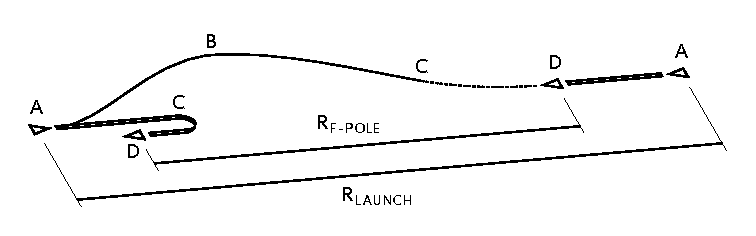
\includegraphics[
            width = 128mm,
    ]{F16_aaweapons_amraam_employment_v07.pdf}
    \caption{Generic, simplified AIM-120 employment profile}
    \label{fig:aaweap:aim120:profile}
\end{figure}

\begin{tcoloritemize}
    \blueitem{Phases}{
    \Cref{fig:aaweap:aim120:profile} shows AIM-120 employment profile
    including the following phases \& milestones

    \begin{subitemize}
        \item \textbf{A} --- Launch
        \item \textbf{B} --- Mid-Course Phase
        \item \textbf{C} --- Acquisition
        \item \textbf{D} --- Intercept
    \end{subitemize}}
    \blueitem{Launch}{
    \textbf{Radar Lock}

    \begin{subitemize}
        \item Only requires track to launch
        \item Target does \textbf{NOT} need to be in STT lock
    \end{subitemize}

%    \textbf{Maximizing Range --- maximizing energy}

%     \begin{subitemize}
%         \item High velocity --- increases kinetic energy
%         \item High altitude --- increases potential energy, reduces drag
%     \end{subitemize}

    \textbf{Lofting} 

    \begin{subitemize}
        \item At longer ranges the missile will loft itself to optimize trajectory
        \item Pilot can manually loft by raising the nose 20-30 deg prior to launch
    \end{subitemize}}
    \blueitem{Mid-Course Phase}{
    \textbf{Missile flies using internal IMU}

    \begin{subitemize}
        \item Receives periodic datalink updates
        \item Will fly to last updated target position if DL lost
    \end{subitemize}}
    \blueitem{Acquisition \& MPRF ``Active'' Phase}{
    Once close to DL bandit location
    \begin{subitemize}
        \item AIM-120 radar turns on in MPRF (Medium Pulse Repetition Frequency) mode 
        \item Locks on to closest / best target
    \end{subitemize}}
    \blueitem{Terminal Phase \& Intercept}{
    Once missile has gone active
    \begin{subitemize}
        \item Flies a PNG intercept trajectory towards the target locked by it's radar 
        \item Requires no further DL support, fighter can now turn away from the bandit
    \end{subitemize}}
\end{tcoloritemize}

\notebox{
    \textbf{Post-Launch Maneuvers}
    \begin{itemize}
            \item For simplicity, \cref{fig:aaweap:aim120:profile} does not show any post-launch maneuvers until point \textbf{C}, where the missile goes active 
            % \item Depending on the tactical situation, it can be beneficial to reduce closure by turning 30-60 deg away from the bandit while maintaing radar contact 
            % \item This can be combined with a dive into thicker air to further reduce bandit missile range and maintain a look-up angle for the radar
    \end{itemize}

    \textbf{Flowing Cold}
    \begin{itemize}
        \item The fighter can turn cold prior to the missile going active
        \item Missile will fly to last DL target position, significantly reducing probability of intercept
    \end{itemize}
}

\warningbox{
    \textbf{AIM-120 HAS \underline{NO} IFF FUNCTIONALITY} --- use caution near friendlies
}

% \clearpage

\subsubsection{TACTICAL CONSIDERATIONS}
\label{subsec:aim120:tactics}

\begin{tcoloritemize}
    \blueitem{Range}{
    \textbf{Fighter-bandit distance} can be measured at different points during the timeline

    \begin{subitemize}
        \item \textbf{R\textsubscript{Launch}} --- distance at launch
        \item \textbf{R\textsubscript{F-Pole}} --- distance at impact
        \item \textbf{R\textsubscript{A-Pole}} --- distance when missile goes active
    \end{subitemize}
    
    \textbf{R\textsubscript{Launch}}, \textbf{R\textsubscript{F-Pole}} are the most relevant and should be maximized. These are visible in \cref{fig:aaweap:aim120:profile}.
    }
    \blueitem{Maximizing Launch Range / Energy}{
    \textbf{Why?}
    \begin{subitemize}
        \item Ability to launch at longer ranges forces bandit defensive
        \item Bandit may not be able to counter-launch
        \item Higher launch energy increases P\textsubscript{intercept} %probability of intercept
    \end{subitemize}
    \textbf{How?}
    \begin{subitemize}
        \item \textbf{High velocity} --- increases kinetic energy 
        \item \textbf{High altitude} --- increases potential energy, reduces drag
    \end{subitemize}}
    \blueitem{Maximizing F-Pole Range}{
    \textbf{Why?}
    \begin{subitemize}
        \item Less likely to enter bandit launch envelope
        \item More time/range to launch 2nd missile if necessary
    \end{subitemize}
    \textbf{How?}
    \begin{subitemize}
        \item \textbf{Crank} --- turn 30-60 degrees away from bandit to reduce closure rate, maintain radar contact
        \item \textbf{Dive} --- reduces threat missile envelope
    \end{subitemize}}
    \blueitem{Flowing Cold}{
    \textbf{Why?}
    \begin{subitemize}
        \item Missile requires no support once active
        \item Defends against unknown missile launches
        \item Further maximizes F-pole range
    \end{subitemize}
    \textbf{How?}
    \begin{subitemize}
        \item \textbf{Turn} --- Away from bandit / threat
        \item \textbf{Dive} --- if necessary, reduces threat missile envelope 
    \end{subitemize}}
    \blueitem{Effect of Bandit Maneuvers}{
    As evident in \cref{fig:aaweap:aim120:profile}, 
    R\textsubscript{Launch} is significantly greater than the distance travelled by the missile
    \begin{subitemize}
        \item DLZ calculated based off \textbf{both} own state \textbf{and} bandit state
        \begin{itemize}
            \item \textbf{Missile is relying on target to keep flying towards us}
        \end{itemize}
        \item Bandit can significantly change missile envelope by reducing closure rate / altitude
        \item If done post-launch can result in missile not having energy to intercept
    \end{subitemize}}
\end{tcoloritemize}

\clearpage

\subsubsection{SYMBOLOGY}

\begin{tcoloritemize}
    \blueitem{Basic Radar Symbology}{For beyond-visual-range radar usage and symbology \textbf{reference \Crefrange{subsec:crm}{subsec:tws}}}
    \blueitem{DLZ}{\textbf{D}ynamic \textbf{L}aunch \textbf{Z}one --- Displays target \& missile range information
    \begin{subitemize}
        \item \textbf{Range Scale}
        \item \textbf{Target Range \& Closure}
        \begin{itemize}
            \item slant range in \underline{nm}
            \item closure rate in \underline{knots}
        \end{itemize}
        \item \textbf{R\textsubscript{aero}} --- Aerodynamic range 
        \begin{itemize}
            \item \underline{maximum kinetic range}
            \item assumes non-maneuvering target
        \end{itemize}
        \item \textbf{R\textsubscript{TR}} --- Turn-and-run range
        \begin{itemize}
            \item maximum range assuming target turns cold at current velocity
        \end{itemize}
        \item \textbf{R\textsubscript{ACT}} --- Active range
        \begin{itemize}
            \item range at which AIM-120 will activate onboard radar
        \end{itemize}
        \item \textbf{R\textsubscript{MIN}} --- Minimum range
        \item \textbf{Countdown}
        \begin{itemize}
            \item \textbf{A} --- seconds until missile goes active
            \item \textbf{T} --- seconds until predicted impact
        \end{itemize}
    \end{subitemize}
    Displayed on both FCR Page \& HUD
    }
    \blueitem{ASC \& ASEC}{Target lead cues to maximize missile performance --- pilot should place \textbf{ASC} inside \textbf{ASEC}
    \begin{subitemize}
        \item \textbf{ASC} --- \textbf{A}ttack \textbf{S}teering \textbf{C}ue
        \item \textbf{ASEC} --- \textbf{A}llowable \textbf{S}teering \textbf{E}rror \textbf{C}ircle
        \begin{itemize}
            \item Dynamically adjusts size based on target maneuvers
            \item Fixed size prior to target designation
        \end{itemize}
    \end{subitemize}
    Displayed on both FCR Page \& HUD
    }
\end{tcoloritemize}

\begin{figure}[htbp]
    \centering
    \fbox{
    \begin{minipage}[t][40mm][t]{100mm}
        \center{\large\textbf{DLZ/ASEC/ASC}}
        \begin{itemize}
            \item show dlz with stuff from text labeled
            \item show combined asc/asec symbology
        \end{itemize}
    \end{minipage}
    }
    \caption{Missile DLZ and ASC/ASEC Symbology}
\end{figure}

\begin{tcoloritemize}
    \blueitem{TLL}{\textbf{T}arget \textbf{L}ocator \textbf{L}ine --- extends from boresight cross towards target, relative angle displayed next to boresight cross}
    \blueitem{Missile Diamond}{Indicates missile seeker line-of-sight}
\end{tcoloritemize}

\begin{figure}[htbp]
    \centering
    \fbox{
    \begin{minipage}[t][75mm][t]{100mm}
        \center{\large\textbf{HUD --- AIM-120 Symbology}}
        \begin{itemize}
            \item show hud in a-a mode, aim-120 selected
            \item label each of the relevant symbology elements explained in text
            \item probably makes sense to have one big figure with all the elements in it just to show what the hud looks like
            \item label additional stuff not mentioned in text
            \begin{itemize}
                \item range/bearing information etc.
            \end{itemize}
        \end{itemize}
    \end{minipage}
    }
    \caption{A-A AIM-120 HUD}
\end{figure}

\begin{tcoloritemize}
    \blueitem{Post-Launch Symbology}{Bugged track symbology is modified to reflect missile launch \& status

    \begin{subitemize}
        \item \textbf{Post-launch} --- Thick ``tail'' is added
        \item \textbf{Post-active} --- Tail begins to flash
        \item \textbf{Post predicted impact} --- Red cross flashes over track
    \end{subitemize}}
\end{tcoloritemize}

\begin{figure}[htbp]
    \centering
    \fbox{
    \begin{minipage}[t][30mm][t]{100mm}
        \center{\large\textbf{MFD --- Post-Launch Symbology}}
        \begin{itemize}
            \item show symbology elements side-by-side
            \item \url{https://forum.dcs.world/topic/279555-purple-fcr-symbology/}
        \end{itemize}
    \end{minipage}
    }
    \caption{Post-Launch Symbology}
\end{figure}


\marginfigeometry

\subsubsection{AIM-120 SELECTION}
\begin{checklistitemize}
    \blueitem{Via A-A Master Mode}{
    \begin{subenumerate}
        \item \textbf{Master Mode} \dotfill \textbf{A-A}
        \item \textbf{SMS OSB 1} \dotfill Verify \textbf{AAM}
        \item \textbf{Selected Weapon} \dotfill Verify \textbf{120C}
        \begin{itemize}
            \item \textbf{SMS OSB 7} --- \textbf{Press}
            \item or \textbf{NWS/MSL STEP} --- \textbf{Press (long)}
        \end{itemize}
    \end{subenumerate}}
    \blueitem{Via MSL OVRD}{
    \begin{subenumerate}
        \item \textbf{DGFT/MSL OVRD} \dotfill \textbf{OVRD}
        \item \textbf{Selected Weapon} \dotfill Verify \textbf{120C} 
        \begin{itemize}
            \item \textbf{SMS OSB 7} --- \textbf{Press}
            \item or \textbf{NWS/MSL STEP} --- \textbf{Press (long)}
        \end{itemize}
    \end{subenumerate}}
    \blueitem{Via DGFT}{
    \begin{subenumerate}
        \item \textbf{DGFT/MSL OVRD} \dotfill \textbf{DGFT}
        \item \textbf{Selected Weapon} \dotfill \textbf{120C}
        \begin{itemize}
            \item \textbf{SMS OSB 7} --- \textbf{Press}
            \item or \textbf{NWS/MSL STEP} --- \textbf{Press (long)}
        \end{itemize}
    \end{subenumerate}}
\end{checklistitemize}

\subsubsection{MADDOG EMPLOYMENT --- NO RADAR}
\begin{checklistenumerate}
    \blueitem{Prerequisites}{
    \begin{subitemize}
        \item \textbf{Selected Weapon} \dotfill \textbf{120C}
        \item \textbf{SLAVE/BORE} \dotfill \textbf{BORE}
        \item \textbf{Master Arm} \dotfill \textbf{ARM}
    \end{subitemize}}
    \blueitem{Fire Missile}{
    \begin{subenumerate}
        \item \textbf{WPN REL} \dotfill \textbf{Depress}
    \end{subenumerate}}
\end{checklistenumerate}

\clearpage

\subsubsection{SINGLE-TARGET EMPLOYMENT}
\label{subsec:aim120:single}
\begin{checklistenumerate}
    \blueitem{Prerequisites}{
    \begin{subitemize}
        \item \textbf{FCR Switch} \dotfill \textbf{FCR}
        \item \textbf{Desired MFD} \dotfill \textbf{FCR Page (SOI)}
        \item \textbf{RF Switch} \dotfill \textbf{NORM}
        \item \textbf{Selected Weapon} \dotfill \textbf{120C}
        \item \textbf{SLAVE/BORE} \dotfill Verify \textbf{SLAVE}
        \item \textbf{Master Arm} \dotfill \textbf{ARM}
    \end{subitemize}}
    \blueitem{CRM Submode}{\textbf{As Desired}
    \begin{subitemize}
        \item \textbf{RWS} --- \textbf{See \Cref{subsec:rws}}
        \begin{itemize}
            \item long-range, fast search
        \end{itemize}
        \item \textbf{TWS} --- \textbf{See \Cref{subsec:tws}}
        \begin{itemize}
            \item dedicated multi-target mode
        \end{itemize}
        \item \textbf{Cycle via}
        \begin{itemize}
            \item \textbf{FCR OSB 2} --- \textbf{Depress}
            \item or \textbf{TMS} --- \textbf{Right (long)}
        \end{itemize}
    \end{subitemize}}
    \blueitem{Radar Acquisition}{%
    \marginpar{
        \captionsetup{type=figure}
        \fbox{
            \begin{minipage}[t][50mm][t]{\marginparwidth}
                \center{\textbf{Bugged/STT Symbology}}
                \begin{itemize}[leftmargin=1em]
                    \item show bugged target symbol
                    \item maybe also show stt symbol?
                \end{itemize}
            \end{minipage}
        }
        \caption{Bugged/STT Symbology}
    }%
    (demonstrated for \underline{RWS})

    \begin{subenumerate}
        \item \textbf{Target} \dotfill under Acquisition cursor
        \item \textbf{TMS} \dotfill \textbf{Forward} (bugged)
    \end{subenumerate}

    If desired can STT lock

    \begin{subenumerate}[start=4]
        \item \textbf{TMS} \dotfill \textbf{Forward} (locked)
    \end{subenumerate}}
    \blueitem{LOS IFF}{%
    \marginpar{
        \captionsetup{type=figure}
        \fbox{
            \begin{minipage}[t][40mm][t]{\marginparwidth}
                \center{\textbf{IFF return}}
                \begin{itemize}[leftmargin=1em]
                    \item maybe show friendly IFF return?
                \end{itemize}
            \end{minipage}
        }
        \caption{IFF return, do not shoot!}
    }%
    \textbf{see \underline{SECTION}}

    \begin{subenumerate}
        \item \textbf{TMS} \dotfill \textbf{Left (long)}
        \item \textbf{IFF Returns} \dotfill \textbf{None} (near target)
        \item \textbf{NCTR ID} \dotfill \textbf{Hostile} (if available)
    \end{subenumerate}}
    \blueitem{Fire Missile}{
    \marginpar{
        \captionsetup{type=figure}
        \fbox{
            \begin{minipage}[t][50mm][t]{\marginparwidth}
                \center{\textbf{AIM-120 DLZ}}
                \begin{itemize}[leftmargin=1em]
                    \item show in-range dlz
                    \item maybe also show asc inside asec?
                \end{itemize}
            \end{minipage}
        }
        \caption{AIM-120 DLZ}
    }
    \begin{subenumerate}
        \item \textbf{ASC} \dotfill within \textbf{ASEC}
        \item \textbf{DLZ} \dotfill indicates \textbf{In-Range}
        \item \textbf{WPN REL} \dotfill \textbf{Depress}
    \end{subenumerate}}
\end{checklistenumerate}

\clearpage

\subsubsection{MULTI-TARGET EMPLOYMENT}
\label{subsec:aim120:multi}

\begin{checklistenumerate}
    \blueitem{Prerequisites}{
    \begin{subitemize}
        \item \textbf{FCR Switch} \dotfill \textbf{FCR}
        \item \textbf{Desired MFD} \dotfill \textbf{FCR Page (SOI)}
        \item \textbf{RF Switch} \dotfill \textbf{NORM}
        \item \textbf{Selected Weapon} \dotfill \textbf{120C}
        \item \textbf{SLAVE/BORE} \dotfill Verify \textbf{SLAVE}
        \item \textbf{Master Arm} \dotfill \textbf{ARM}
    \end{subitemize}}
    \blueitem{CRM Submode}{\textbf{As Desired}
    \begin{subitemize}
        \item \textbf{RWS} --- \textbf{See \Cref{subsec:rws}}
        \begin{itemize}
            \item max 2-target engagement (DTT)
        \end{itemize}
        \item \textbf{TWS} --- \textbf{See \Cref{subsec:tws}}
        \begin{itemize}
            \item dedicated multi-target mode
        \end{itemize}
        \item \textbf{Cycle via}
        \begin{itemize}
            \item \textbf{FCR OSB 2} --- \textbf{Depress}
            \item or \textbf{TMS} --- \textbf{Right (long)}
        \end{itemize}
    \end{subitemize}}
    \blueitem{Radar Acquisition}{(demonstrated for \underline{TWS})
    \marginpar{
        \captionsetup{type=figure}
        \fbox{
            \begin{minipage}[t][60mm][t]{\marginparwidth}
                \center{\textbf{System / Bugged Target Symbology}}
                \begin{itemize}[leftmargin=1em]
                    \item show system / bugged target symbology
                    \item maybe format as a diagram/flow chart?
                    \item maybe combine into one fig wth search/track target fig?
                    \item can reuse from apg68 chapter
                \end{itemize}
            \end{minipage}
        }
        \caption{System / Bugged Target Symbology}
    }
    \begin{subenumerate}
        \item \textbf{Target} \dotfill under \textbf{Acquisition cursor}
        \item \textbf{TMS} \dotfill \textbf{Forward}
    \end{subenumerate}
    
    Or upgrade \underline{all} tracks to system tracks

    \begin{subenumerate}[start=2]
        \item \textbf{TMS} \dotfill \textbf{Right}
    \end{subenumerate}}
    \blueitem{SCAN IFF}{\textbf{see \underline{SECTION}}

    \begin{subenumerate}
        \item \textbf{TMS} \dotfill \textbf{Left (short)}
        \item \textbf{IFF Returns} \dotfill \textbf{None} (near tracks)
    \end{subenumerate}}
    \blueitem{Bug Acquisition}{
    \begin{subenumerate}
        \item \label{subsec:aim120:multi:acq}\textbf{Target} \dotfill under Acquisition cursor
        \item \textbf{TMS} \dotfill \textbf{Forward}
    \end{subenumerate}}
    \blueitem{Fire Missile}{
    \marginpar{
        \captionsetup{type=figure}
        \fbox{
            \begin{minipage}[t][50mm][t]{\marginparwidth}
                \center{\textbf{AIM-120 DLZ}}
                \begin{itemize}[leftmargin=1em]
                    \item show in-range dlz
                    \item maybe also show asc inside asec?
                \end{itemize}
            \end{minipage}
        }
        \caption{AIM-120 DLZ}
    }
    \begin{subenumerate}
        % \item \label{subsec:aim120:multi:acq}\textbf{Target} \dotfill under Acquisition cursor
        % \item \textbf{TMS} \dotfill \textbf{Forward} (bugged)
        \item \textbf{ASC} \dotfill within \textbf{ASEC}
        \item \textbf{DLZ} \dotfill indicates \textbf{In-Range}
        \item \label{subsec:aim120:multi:wpnrel}\textbf{WPN REL} \dotfill \textbf{Depress}
    \end{subenumerate}
    \textbf{Repeat \crefrange{subsec:aim120:multi:acq}{subsec:aim120:multi:wpnrel} for desired targets}
    }
\end{checklistenumerate}

% \notebox{
%     \begin{itemize}
%         \item Bugged target can be cycled in range order with \textbf{TMS Right}
%         \item Similar 2-target employment possible for RWS-DTT mode, \textbf{see \Cref{subsec:rws}}
%     \end{itemize}
% }

\marginfigrestore